\documentclass[professionalfonts]{beamer}
\usepackage{cmap}
\usepackage{fontspec}
\usepackage{lmodern}
\usepackage{microtype}
\usepackage[english]{babel}
\usepackage{tikz}
\usepackage{minted}
\usepackage{xcolor}

\usetheme{AnnArbor}
\usecolortheme{spruce}
\setbeamercolor{button}{bg=black, fg=yellow}

\usetikzlibrary{positioning}
\usetikzlibrary{calc}

\title{Lustrean}
\subtitle{Lustre + Lean = Lustrean}
\author{Jean \textsc{Caspar} \and Adrien \textsc{Mathieu}}
\date{December 2024}

\makeatletter
\newcommand*{\currentname}{\@currentlabelname}
\def\ft{\frametitle{\currentname}}
\makeatother

\setbeamertemplate{itemize items}[square]
\setbeamertemplate{enumerate items}[default]

% \newfontfamily\NHLight[ItalicFont = HelveticaNeueLT Std Thin]{Helvetica Neue LT Std}
\newcommand\textulf[1]{{
    %\NHLight
    \textit#1}}

\newcommand{\lustrean}[1]{\scalebox{#1}{%
  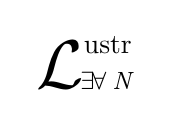
\begin{tikzpicture}%
    \node (L) {\Huge\(\mathcal{L}\)};%
    \node at (.6,.25) {ustr};%
    \node at (.6,-.2) {\small ${\exists}\hspace*{-.1em}{\forall}$\hspace*{-.1em}\raisebox{-.05ex}{\textulf{N}}};%
  \end{tikzpicture}%
}}

\begin{document}

\begingroup
\setbeamertemplate{headline}{}
\setbeamertemplate{footline}{}
\begin{frame}[noframenumbering]
  \titlepage
\end{frame}
\endgroup

\section{Overview}
\subsection{Lustrean}
\begin{frame}
  \ft{}
  \begin{center}
    \lustrean{2}
  \end{center}
  Lustrean is an abstract interpreter of a precise semantics of a core subset of Lustre in Lean.
  \begin{itemize}
  \item It embeds a subset of Lustre as a DSL in Lean.
  \item It gives a precise semantics of that language, even to non-statically schedulable programs.
  \item It interprets them in an abstract domain to check for the absence of runtime errors.
  \end{itemize}
\end{frame}

\subsection{Lustre embedding}
\begin{frame}
  \ft{}

  The embedding of Lustre into Lean works by progressively collapsing the language into simpler
  and simpler languages, by iterating simple atomic phases:
  \begin{itemize}
  \item syntax analysis;
  \item reification;
  \item inlining;
  \item ``indicisation'';
  \item normalization.
  \end{itemize}
\end{frame}

\subsection{Precise semantics}
\begin{frame}[fragile]
  \ft{}

  We aim at accepting the following program
  \begin{verbatim}
node f(c, z) = y where
  y = if c then x else z
  x = if c then z else y
  \end{verbatim}
  which cannot be statically scheduled.  It is, however, always possible to find, depending on
  the value of \texttt{c}, an order to evaluate these equations that makes everything
  well-defined.

  We therefore interpret this program with values in the flat domain \(\mathbb{N} + \{nil\}\),
  with ordering \(nil \leq n\) for \(n\in\mathbb{N}\).

  We initialize every value at \(nil\), and then iterate the equations until it converges.  This
  fails if an output variable still contains the value \(nil\).
\end{frame}

\subsection{Abstracting the semantics}
\begin{frame}
  \ft{}


\end{frame}

\section{Abstract domains}
\subsection{Domain}
\begin{frame}
  \ft{}
  A domain over $n$ variables a data structure
  which represents an overapproximation of a
  set of environments. It has:

  \begin{itemize}
  \item decidable equality,
  \item a function which returns a new environment,
  \item an assignation function which takes an integer expression and updates the environment
    accordingly,
  \item a guard function which takes a boolean expression and refines the environment to keep
    only those states that makes the boolean exwhich should be different from $\bot$.pression be
    true,
  \item a widening and a narrowing operators.
  \end{itemize}

  The code is inspired from the TP of abstract interpretation
  from Antoine Miné, Marc Chevalier and Josselin Giet.
\end{frame}

\subsection{Non relational domain}
\begin{frame}
  \ft{}
  A non relational domain is a domain of the form
  $\{0, \dots, n-1\} \to V$ where $V$ is a domain
  representing values.

  The value domains are bounded lattice with a widening
  and a narrowing which support arithmetic operations.

  We did not use any relational domains, as it would have
  been to long to implement and to prove properties on them.
\end{frame}

\subsection{Nil in values domains}
\begin{frame}
  \ft{} Values domains are also required to contain an element representing $nil$. The order of
  the lattice is an order represeting the set of possible values the expression can take ; it is
  not the order ``x is less defined than y''. Especially, we do not have $nil \sqsubseteq 3$.

  This is different than in the domain used in the concrete semantics, where we do have
  \(nil \leq 3\).
\end{frame}

\subsection{Concrete value domains}
\begin{frame}
  \ft{}

  \begin{itemize}
  \item Integers with a top and bottom element.
  \item Intervals.
  \end{itemize}
  These domains send nil to top.
  \begin{itemize}
  \item A domain combinator which transform a domain $D$ into $D \times \mathbb{B}$, where
    $(v, \operatorname{false})$ represents the set of values represented by $v$, except $nil$,
    and $(v, \operatorname{true})$ represents the set of values represented by $v$ and $nil$.
  \end{itemize}
\end{frame}

\section{Interpreter}
\subsection{CFG}
\begin{frame}
  \ft{}
  \begin{itemize}
  \item The interpreter is given a list of ``pre nodes'', parameterized by the number of
    variables.
  \item A pre node is a list of tuples $(inst, out, synt)$.
  \item $inst$ is an instruction, $out$ the index of the exit node as a natural number, $synt$ a
    pointer to the piece of code from which the instruction originates.
  \end{itemize}
\end{frame}

\begin{frame}
  \ft{}
  \begin{itemize}
  \item We compile the pre nodes to a cfg. It consists of an array of nodes and arcs.
  \item An arc contains an instruction, the index of the source node and of the exit node, and a
    pointer to the syntax.
  \item A node contains the list of the indices of the arcs going into it.
  \end{itemize}
  Indices lives in \texttt{Fin arcs.size}, respectively \texttt{Fin nodes.size}.

  Because we have to translate the first representation into the second while
  assuring correctness, there is a lot of bookkeeping
  involved with dependent types, and I used
  no less that two intermediate structures.

  We also compute a set of widening points, which select at least
  one node in each strongly connected component of the cfg.
\end{frame}

\subsection{Execution}
\begin{frame}
  \ft{}
  \begin{itemize}
  \item After that, we build a state which assigns a environment (living in a domain) to each
    node and arc.
  \item First we iterate over all arcs and assigns to each arc the value of the transfer function
    of this arc to the source environment.
  \item Then we iterate over the nodes and assigns to the them the union of the environments of
    their entrant arcs. If the node is a widening point, we perform a widening.
  \item We currently don't use the narrowing.
  \item When it stabilizes, we return the state.
  \end{itemize}
\end{frame}

\section{Monads and dependent types}
\subsection{Indicisation}
\begin{frame}
  \ft{}
\end{frame}

\subsection{Normalization}
\begin{frame}
  \ft{}
\end{frame}

\section{Possible improvements}
\subsection{Domain partitioning}
\begin{frame}
  \ft{}
  For an \(m\in\mathbb{N}\), partitioning along \(n = k\) for \(k<m\) and \(n \geq m\).
  Chose \(m\) to be the maximally nested \texttt{pre} occurrences.
\end{frame}

\subsection{Partial scheduling}
\begin{frame}
  \ft{} We cannot statically schedule equations in the general case, yet if we could, this would
  greatly speed up convergence: in the precise semantics, if the equations can be scheduled, and
  if they are executed while being scheduled it takes \(O(n)\) time to compute them, and not
  \(O(n^2)\) time as in the general case.

  More generally, if we do a partial topological sort, the convergence complexity of a single
  step becomes \(O(nk)\) where \(k\) is the size of largest dependency cycle.
\end{frame}

\subsection{Separation of semantics}
\begin{frame}
  \ft{}

  Currently, there is no intermediate representation that corresponds to the concrete semantics:
  the language is compiled right away into its abstract semantics.  This means that we cannot
  reason in Lean just about the concrete semantics.

  If we isolated these concrete semantics, and proved soundness of our abstraction, we could turn
  our abstract interpreter into a tactic that tries to automatically prove the absence of runtime
  errors of a Lustre program, on which we could otherwise reason, and that we could extract into
  a standalone program.
\end{frame}

\section{Correctness}
\begin{frame}
  \ft{}
  \begin{itemize}
  \item The notion of domain is totally formalized, save for the termination property of the
    narrowing and of the widening: we need classical logic to prove it, but then it would be
    difficult to extract the witness.
  \item We didn't provide a concrete semantics and proved that the abstract semantics is a sound
    abstraction of the concrete semantics.
  \item We don't have an other semantics to which we can compare our interpreter and relatively
    to which we can prove soundness.
  \item The array accesses are all proven correct.
  \end{itemize}
\end{frame}

\end{document}
